\documentclass[tikz,border=5pt]{standalone}
\usepackage{amsmath}
\usetikzlibrary{arrows,calc}

\definecolor{obsfill}{HTML}{EBF1F7}
\definecolor{obsdraw}{HTML}{4C78A8}
\definecolor{basefill}{HTML}{F0F0F0}
\definecolor{basedraw}{HTML}{8C8C8C}
\definecolor{resfill}{HTML}{FDF3E7}
\definecolor{resdraw}{HTML}{E08E2B}
\definecolor{teal}{HTML}{2A9D8F}
\definecolor{corrfill}{HTML}{EEF6ED}
\definecolor{corrdraw}{HTML}{59A14F}
\definecolor{evalfill}{HTML}{F4F5F7}
\definecolor{charcoal}{HTML}{3A3A3A}
\definecolor{provenance}{HTML}{555555}

\newcommand{\moduleheader}[1]{%
  {\sffamily\fontsize{9.5}{11}\selectfont\bfseries #1}}
\newcommand{\mathtext}{\fontsize{8.5}{11}\selectfont}

\begin{document}
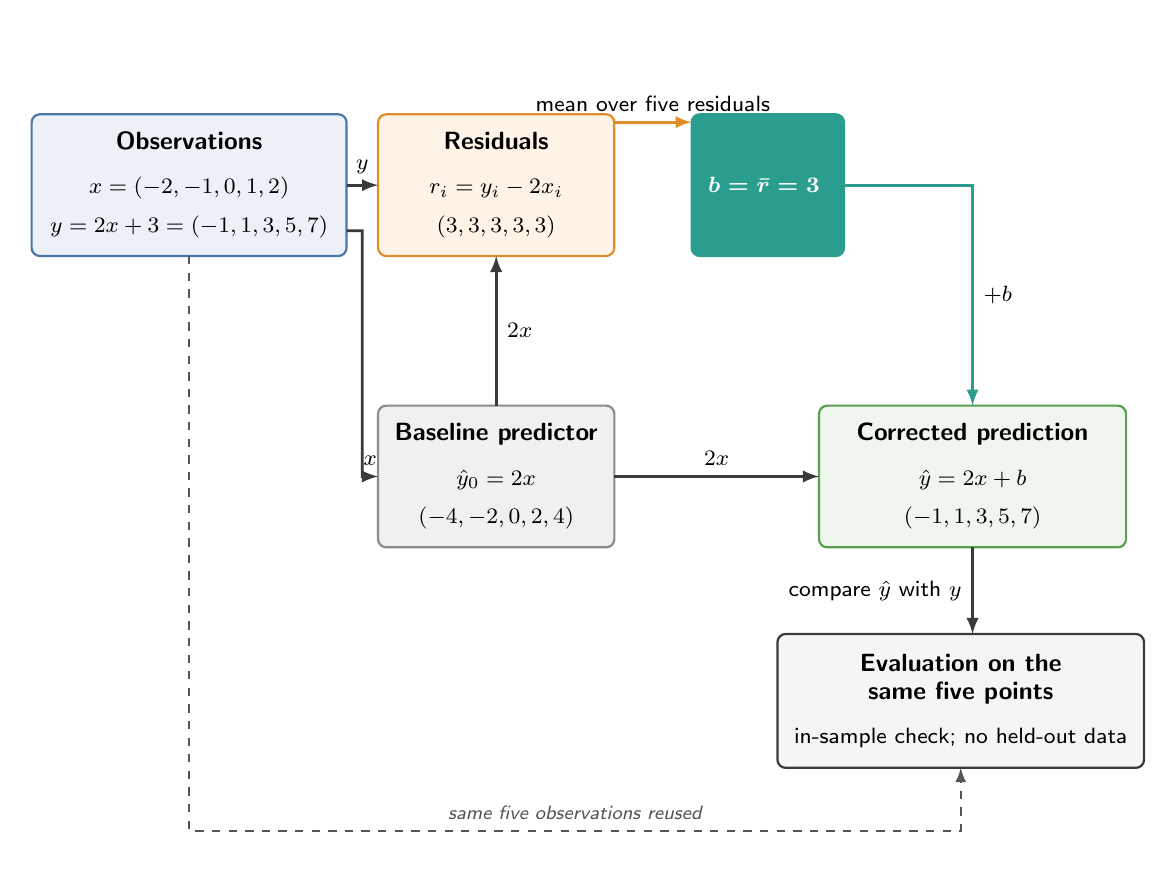
\begin{tikzpicture}[
  box/.style={
    rectangle,
    rounded corners=3pt,
    line width=0.8pt,
    inner xsep=6pt,
    inner ysep=6pt,
    outer sep=0pt,
    align=center,
    font=\mathtext
  },
  flow/.style={
    -latex,
    line width=1pt,
    draw=charcoal,
    line cap=butt,
    line join=miter
  },
  reuse/.style={
    -latex,
    line width=0.8pt,
    dashed,
    draw=provenance,
    line cap=butt,
    line join=miter
  },
  mathlabel/.style={
    font=\fontsize{8}{10}\selectfont,
    inner sep=0pt,
    outer sep=0pt,
    fill=white
  },
  textlabel/.style={
    font=\sffamily\fontsize{8}{10}\selectfont,
    inner sep=0pt,
    outer sep=0pt,
    fill=white,
    align=center
  }
]

% White 4:3 canvas.
\path[fill=white] (0,0) rectangle (14,10.5);
\path[use as bounding box] (0,0) rectangle (14,10.5);

% Column 1: observations.
\node[
  box,
  draw=obsdraw,
  fill=obsfill,
  minimum width=4cm,
  minimum height=1.8cm
] (D1) at (2.05,8.5) {
  \moduleheader{Observations}\\[5pt]
  $x=(-2,-1,0,1,2)$\\[3pt]
  $y=2x+3=(-1,1,3,5,7)$
};

% Column 2: residuals and baseline prediction.
\node[
  box,
  draw=resdraw,
  fill=resfill,
  minimum width=3cm,
  minimum height=1.8cm
] (R) at (5.95,8.5) {
  \moduleheader{Residuals}\\[5pt]
  $r_i=y_i-2x_i$\\[3pt]
  $(3,3,3,3,3)$
};

\node[
  box,
  draw=basedraw,
  fill=basefill,
  minimum width=3cm,
  minimum height=1.8cm
] (B) at (5.95,4.8) {
  \moduleheader{Baseline predictor}\\[5pt]
  $\hat{y}_0=2x$\\[3pt]
  $(-4,-2,0,2,4)$
};

% Column 3: scalar intercept correction.
\node[
  box,
  draw=teal,
  fill=teal,
  text=white,
  minimum width=1.5cm,
  minimum height=1.8cm
] (S) at (9.4,8.5) {
  {\boldmath $b=\bar{r}=3$}
};

% Column 4: corrected prediction and evaluation.
\node[
  box,
  draw=corrdraw,
  fill=corrfill,
  minimum width=3.9cm,
  minimum height=1.8cm
] (C) at (12,4.8) {
  \moduleheader{Corrected prediction}\\[5pt]
  $\hat{y}=2x+b$\\[3pt]
  $(-1,1,3,5,7)$
};

\node[
  box,
  draw=charcoal,
  fill=evalfill,
  minimum width=4.1cm,
  minimum height=1.7cm
] (E) at (11.85,1.95) {
  \moduleheader{Evaluation on the}\\[-1pt]
  \moduleheader{same five points}\\[5pt]
  {\sffamily\fontsize{8.5}{11}\selectfont
   in-sample check; no held-out data}
};

% Target observations enter the residual calculation.
\draw[flow] (D1.east) -- (R.west)
  node[midway,above=4pt,mathlabel] {$y$};

% Predictor input: a separate orthogonal branch.
\coordinate (xexit) at ($(D1.south east)+(0,0.32)$);
\draw[flow]
  (xexit) -- (4.25,7.92) -- (4.25,4.8) -- (B.west)
  node[pos=0.5,above=4pt,mathlabel] {$x$};

% Baseline prediction enters the residual calculation.
\draw[flow] (B.north) -- (R.south)
  node[midway,right=4pt,mathlabel] {$2x$};

% The upper-flank connection leaves room for its single-line label.
\coordinate (meanstart) at ($(R.north east)+(0,-0.1)$);
\coordinate (meanend) at ($(S.north west)+(0,-0.1)$);
\draw[flow,draw=resdraw] (meanstart) -- (meanend)
  node[midway,above=4pt,textlabel] {mean over five residuals};

% Baseline prediction is carried directly into the corrected prediction.
\draw[flow] (B.east) -- (C.west)
  node[midway,above=4pt,mathlabel] {$2x$};

% Scalar correction enters the top of the corrected-prediction module.
\draw[flow,draw=teal]
  (S.east) -- (12,8.5) -- (C.north)
  node[midway,right=4pt,mathlabel] {$+b$};

% In-sample comparison.
\coordinate (evaluationentry) at (C.south |- E.north);
\draw[flow] (C.south) -- (evaluationentry)
  node[midway,left=4pt,textlabel]
  {compare $\hat{y}$ with $y$};

% Provenance: the original observations are reused for evaluation.
\coordinate (reusebottom) at ($(E.south)+(0,-0.8)$);
\draw[reuse]
  (D1.south)
  -- (D1.south |- reusebottom)
  -- (reusebottom)
  -- (E.south);

\node[
  font=\sffamily\itshape\fontsize{7.5}{9}\selectfont,
  text=provenance,
  fill=white,
  inner sep=0pt,
  anchor=south
] at ($(D1.south |- reusebottom)!0.5!(reusebottom)+(0,4pt)$)
  {same five observations reused};

\end{tikzpicture}
\end{document}